

\arrayrulecolor{Couleur6}

\chapter{Équations de droites et systèmes d'équations}



\section{Équation cartésienne d'une droite}
Dans tout le chapitre, le plan est muni d'un repère orthonormé $(O;\overrightarrow{i},\overrightarrow{j})$.

\begin{Définition}
On appelle vecteur directeur d'une droite $d$ tout vecteur non nul dont la direction est celle de $d$.

\end{Définition}

\begin{Remarque}
Une droite a une infinité de vecteurs directeurs, tous colinéaires.\\
Si $A$ et $B$ sont deux points distincts de la droite $d$, alors le vecteur $\overrightarrow{AB}$ est un vecteur directeur de $d$.
\end{Remarque}

\begin{Propriété}

Toute droite $d$ a une équation de la forme $ax+by+c=0$, avec $(a;b)\neq(0;0)$ appelée {\bf{équation cartésienne}} de $d$.
Le vecteur $\overrightarrow{u}\begin{pmatrix}
-b \\
a
\end{pmatrix}$ est un vecteur directeur de $d$.


\end{Propriété}

\begin{proof}
$ \\ $
Soit $d$ la droite passant par le point $A(x_A;y_A)$ et de vecteur directeur $\overrightarrow{u}\begin{pmatrix}
\alpha \\
\beta
\end{pmatrix}$.\\
Le point $M$ de coordonnées $(x;y)$ appartient à $d$ si, et seulement si, $\overrightarrow{AM}$ et $\overrightarrow{u}$ sont colinéaires, ce qui équivaut à $\begin{vmatrix}
x-x_A & \alpha \\
y-y_A & \beta
\end{vmatrix}=0$. Cela équivaut à $\beta(x-x_A)-\alpha(y-y_A)=0$, soit $\beta x -\alpha y -\beta x_A +\alpha y_A=0$. \\
Cette équation est de la forme $ax+by+c=0$ avec $a=\beta$, $b=-\alpha$ et $c=-\beta x_A +\alpha y_A$. \\
Ainsi, $\begin{pmatrix}
\alpha \\
\beta
\end{pmatrix}=\begin{pmatrix}
-b \\
a
\end{pmatrix}$; donc un vecteur directeur de $d$ est $\overrightarrow{u}\begin{pmatrix}
-b \\
a
\end{pmatrix}$. \\Or, un vecteur directeur est non nul, donc $(a;b)\neq(0;0)$.

\end{proof}

\vspace{-0.5cm}


\begin{Exemple}
On considère la droite $(d)$ qui passe par le point $A$ de coordonnées $(5\,;\,-1)$ et qui a le vecteur $\vec u \begin{pmatrix}1\\2\end{pmatrix}$ comme vecteur directeur. Déterminer une équation cartésienne de la droite $(d)$.
\vspace{0.1cm}

\ligne

\ligne

\ligne

\ligne

\ligne

\ligne

\ligne

\ligne

\end{Exemple}


\begin{Remarque}
Une droite a une infinité d'équations cartésiennes. À partir d'une, on peut obtenir les autres en multipliant par le même réel non nul les coefficients $a$, $b$, et $c$.
\end{Remarque}


\begin{Exemple}
L'ensemble des points $M(x;y)$ tels que $2x-3y+1=0$ est une droite $d$ de vecteur directeur $\overrightarrow{u}\begin{pmatrix}
3 \\
2
\end{pmatrix}$. 
\vspace{0.1cm}

\ligne

\ligne

\end{Exemple}

\paragraph{Cas particuliers : $a=0$ et $b=0$}
\begin{itemize}[label=\textcolor{Couleur8}{$\bullet$}]
\item Une droite d'équation $y=k$ est une droite parallèle à l'axe des abscisses. \\Un de ses vecteurs directeurs est $\overrightarrow{i}\begin{pmatrix}
1\\
0
\end{pmatrix}$.
\item  Une droite d'équation $x=k$ est une droite parallèle à l'axe des ordonnées. \\Un de ses vecteurs directeurs est $\overrightarrow{j}\begin{pmatrix}
0\\
1
\end{pmatrix}$.
\end{itemize}



\section{Équation réduite d'une droite}

\subsection{Rappels}
\begin{minipage}[c]{0.5\linewidth}
\noindent Soit $d$ une droite d'équation réduite $y=mx+p$. \\
Soit $A(x_A;y_A)$ et $B(x_B;y_B)$\\
$m$ est la coefficient directeur et $m=\dfrac{y_B-y_A}{x_B-x_A}$.\\
$p$ est l'ordonnée à l'origine.
\end{minipage} \hfill
\begin{minipage}[c]{0.5\linewidth}
\begin{center}
\vspace{-0.8cm}
\begin{tikzpicture}[x=0.7cm,y=0.5cm]
% Définition des limites
\def\xmin{-3}
\def\xmax{6}
\def\ymin{-1}
\def\ymax{6}

% Grille en pointillés
\draw[dotted, gray] (\xmin,\ymin) grid[step=1] (\xmax,\ymax);

% Axes
\draw[->,thick] (\xmin,0) -- (\xmax,0) node[below right] {$x$};
\draw[->,thick] (0,\ymin) -- (0,\ymax) node[above left] {$y$};

% Labels des axes
\draw (0,0) node[below left] {0};
\draw (1,0) node[below] {1};
\draw (0,1) node[left] {1};

% Droite Couleur10
\draw[samples=300,domain=-3:6,Couleur10,thick] plot(\x,{-0.6*\x+2.8});

% Point p sur la droite (intersection avec l'axe y)
\draw[Couleur10] (0,2.8) node {$\times$};
\draw[Couleur10] (-0.7,2.5) node {$p$};

% Label de la droite
\draw[Couleur10] (4.33,-0.1) node[anchor=north west] {$d$};

% Points A et B
\draw[Couleur1] (-2,4.5) node {$A$};
\draw[Couleur1] (3,0.5) node {$B$};

% Flèches bleues pour montrer les différences
\draw[Couleur6,->] (-2,4) -- (3,4);
\draw[Couleur6,->] (3,4) -- (3,1);

% Labels pour les différences
\draw[Couleur6] (0.5,4.5) node {$x_B-x_A$};
\draw[Couleur6] (4.5,2.5) node {$y_B-y_A$};

% Formule de la pente
\draw[Couleur6] (3.8,4.8) node {$m=\dfrac{y_B-y_A}{x_B-x_A}$};

\end{tikzpicture}
\end{center}
\end{minipage}


\begin{Exemple}
Déterminer une équation réduite de la droite $(AB)$ avec $A(3\,;\,4)$ et $B(7\,;\,-5)$. 
\vspace{0.1cm}

\ligne

\ligne

\ligne

\ligne

\ligne

\ligne

\ligne

\ligne

\end{Exemple}

\subsection{Lien entre l'équation cartésienne et l'équation réduite}
\begin{Méthode}Passer d'une équation à l'autre. \\
Soit $d$ une droite non parallèle à l'axe des ordonnées d'équation cartésienne $ax+by+c=0$ et d'équation réduite $y=mx+p$. \\
On a donc $b\neq 0$ (non parallèle à l'axe des ordonnées).\\
Alors $y=\dfrac{-a}{b}+\dfrac{-c}{b}$. Ainsi, $m=\dfrac{-a}{b}$ et $p=\dfrac{-c}{b}$.\\
Si $b=0$, alors $ax+c=0$ donc $x=\dfrac{-c}{a}$ est une droite parallèle à l'axe des ordonnées.
\end{Méthode}

\begin{Propriété}
Soit $d$ une droite d'équation réduite $y=mx+p$ alors $\overrightarrow{u}\begin{pmatrix}
1 \\
m\end{pmatrix}$ est un vecteur directeur de la droite $d$.
\end{Propriété}

\begin{proof}
On a $d$ qui s'écrit aussi $ax+by+c=0$ avec $b\neq 0$ et $m=\dfrac{-a}{b}$ et $p=\dfrac{-c}{b}$.\\
Or, $\overrightarrow{v}\begin{pmatrix}
-b \\
a \end{pmatrix}$ est un vecteur directeur de la droite $d$. \\
Comme $b\neq 0$, $\overrightarrow{u}=\dfrac{-1}{b}\times\overrightarrow{v}\begin{pmatrix}
1 \\
\dfrac{-a}{b}\end{pmatrix}=\begin{pmatrix}
1 \\
m\end{pmatrix}$ est aussi un vecteur directeur de la droite $d$. 
\end{proof}
\newpage

\section{Systèmes de deux équations linéaires à deux inconnues}

\begin{Définition}
Un système de deux équations linéaires du premier degré à deux inconnues $x$ et $y$ est de la forme $\left\{
    \begin{array}{ll}
     ax+by=c    & \\
       a'x+b'y=c' & 
    \end{array}
\right.$, où $a,b,c,a',b'$ et $c'$ sont des réels et $(x;y)$ le couple des inconnues.

\end{Définition}

\begin{Remarque}
\noindent {\bf{Résoudre}} ce système revient à {\bf{déterminer tous les couples solutions}}, c'est à dire tous les couples vérifiant {\bf{simultanément }} les deux équations du système. 
\end{Remarque}

\begin{Exemple}
Soit le système $\left\{
    \begin{array}{ll}
     3x-2y=6    & \\
       -4x+5y=-1 & 
    \end{array}
\right.$.
\vspace{0.3cm}

\ligne

\end{Exemple}

\begin{Méthode}Par substitution. \\
Résoudre le système 
$(S)\left\{
    \begin{array}{ll}
     3x-y=5    & \\
       2x+3y=7 & 
    \end{array}
\right.$

\vspace{0.3cm}

\ligne

\ligne

\ligne

\ligne

\ligne

\ligne

\ligne

\ligne

\ligne

\ligne

\end{Méthode}


\begin{Méthode}Par combinaison. \\

Résoudre le système 
$(S)\left\{
    \begin{array}{ll}
     2x-5y=1    & \\
       3x+2y=11 & 
    \end{array}
\right.$ 
\vspace{0.3cm}

\ligne

\ligne

\ligne

\ligne

\ligne

\ligne

\ligne

\ligne

\ligne

\begin{Remarque}
On peut aussi soustraire les deux équations termes à termes en multipliant par Exemple, la première équation par $3$ et la deuxième par $2$ et en faisant la première moins la deuxième pour supprimer les $x$.
\end{Remarque}

\end{Méthode}
\newpage

\section{Parallélisme et intersection de deux droites}

\begin{Définition}$ $ 
\begin{itemize}[label=\textcolor{Couleur6}{$\bullet$}]
\item Deux droites $d$ et $d'$ sont {\bf{parallèles}} quand elles ont la même direction.
\item Deux droites non parallèles sont dites {\bf{sécantes}}.
\end{itemize}

\end{Définition}



\begin{Propriété}
Deux droites $d$ et $d'$ sont parallèles si, et seulement si, deux de leurs vecteurs directeurs sont colinéaires.
\end{Propriété}

\begin{Exemple}
Soit $d$ et $d'$ des droites d'équations respectives $4x-2y=0$ et $-12x+6y-3=0$. Sont-elles parallèles ?
\vspace{0.1cm}

\ligne

\ligne

\ligne

\ligne

\ligne

\end{Exemple}

\begin{Propriété}
Deux droites $d$ et $d'$ d'équations réduites $y=mx+p$ et $y=m'x+p'$ sont parallèles si, et seulement si, leurs pentes sont égales $m=m'$.
\end{Propriété}
\vspace{-0.5cm}
\begin{proof}
$\overrightarrow{u}\begin{pmatrix}
1\\
m
\end{pmatrix}$ est un vecteur directeur de $d$ et  $\overrightarrow{v}\begin{pmatrix}
1\\
m'
\end{pmatrix}$ est un vecteur directeur de $d'$.\\
Ainsi, les droites $d$ et $d'$ sont parallèles si, et seulement si, les vecteurs $\overrightarrow{u}$ et $\overrightarrow{v}$ sont colinéaires, ce qui équivaut à $\det(\overrightarrow{u},\overrightarrow{v})=\begin{vmatrix}
1 & 1\\
m & m'
\end{vmatrix}= m'-m=0$, c'est à dire $m'=m$. 
\end{proof}

\begin{Remarque}
Deux droites confondues sont parallèles et elles ont des équations cartésiennes multiples l'une de l'autre.\\
$x-2y+1=0$ et $4x-8y+4=0$ sont les équations cartésiennes de 2 droites confondues, car $4(x-2y+1)=4x-8y+4$.
\end{Remarque}


\begin{Propriété} $ $
\begin{itemize}[label=\textcolor{Couleur2}{$\bullet$}]
\item Si deux droites $d$ et $d'$ sont sécantes, alors les coordonnées de leur point d'intersection est l'unique couple solution du système formé par une équation de $d$ et une équation de $d'$.
\item Résoudre le système $(S)\left\{
    \begin{array}{ll}
     ax+by=c    & \\
       a'x+b'y=c' & 
    \end{array}
\right.$, revient à étudier l'intersection de deux droites du plan.\\ 
Le système $(S)$ admet soit une unique solution, soit aucune solution, soit une infinité de solutions.
\end{itemize}
\end{Propriété}

\begin{center}
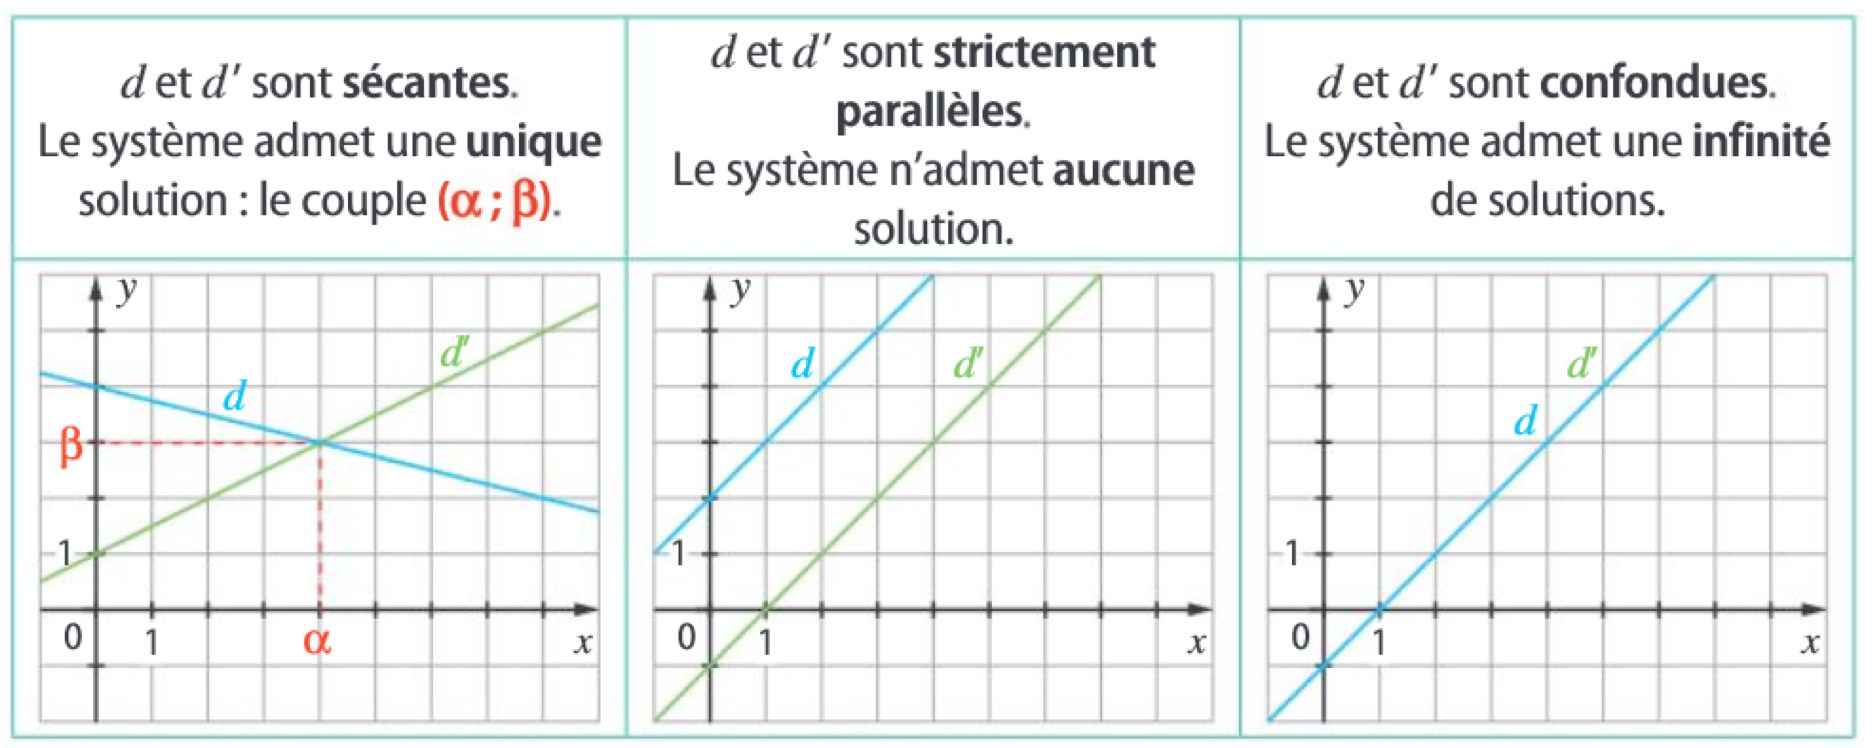
\includegraphics[scale=.45]{IMG/intersection_chap_11}
\end{center}

\bigskip

\newpage

\section*{Exercices - Équations de droites et systèmes d'équations}
\addcontentsline{toc}{section}{Exercices}
{\setlength{\columnseprule}{0pt}
\setcounter{NumEx}{1}


\subsection*{Équations de droites}

% @see : https://coopmaths.fr/alea?uuid=1bb30&id=2G30-3&n=8&d=10&s=2&alea=yD3m&cd=1&cols=2
\begin{Exercice}
Déterminer une équation cartésienne de la droite $(AB)$ où :.
\vspace{-0.5cm}
\begin{multicols}{2}
\begin{enumerate}[itemsep=1em]
\item \begin{minipage}[t]{\linewidth} Avec $A(-2\,;\,-4)$ et $B(0\,;\,-1)$.. \end{minipage}
	\item \begin{minipage}[t]{\linewidth} Avec $A(3\,;\,2)$ et $B(5\,;\,3)$.. \end{minipage}
	\item \begin{minipage}[t]{\linewidth} Avec $A(0\,;\,-5)$ et $B(-4\,;\,5)$.. \end{minipage}
	\item \begin{minipage}[t]{\linewidth} Avec $A(4\,;\,-3)$ et $B(5\,;\,-4)$.. \end{minipage}
	\item \begin{minipage}[t]{\linewidth} Avec $A(-5\,;\,-5)$ et $B(-1\,;\,-2)$.. \end{minipage}
	\item \begin{minipage}[t]{\linewidth} Avec $A(4\,;\,3)$ et $B(2\,;\,5)$.. \end{minipage}
	\item \begin{minipage}[t]{\linewidth} Avec $A(2\,;\,-4)$ et $B(0\,;\,4)$.. \end{minipage}
	\item \begin{minipage}[t]{\linewidth} Avec $A(-3\,;\,-5)$ et $B(1\,;\,1)$.. \end{minipage}
\end{enumerate}
\end{multicols}
\end{Exercice}

% @see : https://coopmaths.fr/alea?uuid=0ec77&id=2G30-4&n=4&d=10&s=1&alea=DdbA&cd=1&cols=2
\begin{Exercice}
Déterminer une équation cartésienne de la droite $(d)$.
\vspace{-0.5cm}
\begin{multicols}{2}
\begin{enumerate}[itemsep=1em]
\item \begin{minipage}[t]{\linewidth} La droite $(d)$ qui passe par le point $A$ de coordonnées $(0\,;\,-2)$ et qui a le vecteur $\vec u \begin{pmatrix}4\\-1\end{pmatrix}$ comme vecteur directeur.\end{minipage}
	\item \begin{minipage}[t]{\linewidth} La droite $(d)$ qui passe par le point $A$ de coordonnées $(4\,;\,-5)$ et qui a le vecteur $\vec u \begin{pmatrix}-2\\-2\end{pmatrix}$ comme vecteur directeur.\end{minipage}
	\item \begin{minipage}[t]{\linewidth} La droite $(d)$ qui passe par le point $A$ de coordonnées $(-1\,;\,5)$ et qui a le vecteur $\vec u \begin{pmatrix}5\\-3\end{pmatrix}$ comme vecteur directeur.\end{minipage}
	\item \begin{minipage}[t]{\linewidth} La droite $(d)$ qui passe par le point $A$ de coordonnées $(1\,;\,-3)$ et qui a le vecteur $\vec u \begin{pmatrix}3\\-1\end{pmatrix}$ comme vecteur directeur.\end{minipage}
\end{enumerate}
\end{multicols}
\end{Exercice}

% @see : https://coopmaths.fr/alea?uuid=d1da3&id=2G30-5&n=4&d=10&s=1&alea=MpUy&cd=1&cols=2
\begin{Exercice}
\leavevmode\vspace{-\baselineskip}
\vspace{-0.5cm}
\begin{multicols}{2}
\begin{enumerate}[itemsep=1em]
	\item \begin{minipage}[t]{\linewidth}Soit $A(3;-3)$ un point d'un repère $(O ; \overrightarrow{i} ;\overrightarrow{j})$.\\Déterminer une équation cartésienne de la droite$(d)$ passant par le point $A$ et ayant pour coefficent directeur $-4$.\end{minipage}
	\item \begin{minipage}[t]{\linewidth}Soit $A(0;5)$ un point d'un repère $(O ; \overrightarrow{i} ;\overrightarrow{j})$.\\Déterminer une équation cartésienne de la droite$(d)$ passant par le point $A$ et ayant pour coefficent directeur $-2$.\end{minipage}
	\item \begin{minipage}[t]{\linewidth}Soit $A(-3;3)$ un point d'un repère $(O ; \overrightarrow{i} ;\overrightarrow{j})$.\\Déterminer une équation cartésienne de la droite$(d)$ passant par le point $A$ et ayant pour coefficent directeur $3$.\end{minipage}
	\item \begin{minipage}[t]{\linewidth}Soit $A(-1;2)$ un point d'un repère $(O ; \overrightarrow{i} ;\overrightarrow{j})$.\\Déterminer une équation cartésienne de la droite$(d)$ passant par le point $A$ et ayant pour coefficent directeur $1$.\end{minipage}
\end{enumerate}
\end{multicols}
\end{Exercice}

\newpage

% @see : https://coopmaths.fr/alea?uuid=1ea16&id=2G30-1&n=9&d=10&s=1&alea=HHBN&cd=1&cols=2
\begin{Exercice}
Soit $\big(O,\vec i;\vec j\big)$ un repère orthogonal.  Déterminer, s'il existe et en l'expliquant, le coefficient directeur de la droite $(AB)$.
\begin{multicols}{3}
\begin{enumerate}[itemsep=1em]
	\item \begin{minipage}[t]{\linewidth}Avec $A(1;-4)$ et $B(-2;-5)$. \end{minipage}
	\item \begin{minipage}[t]{\linewidth}Avec $A(1;1)$ et $B(-5;5)$. \end{minipage}
	\item \begin{minipage}[t]{\linewidth}Avec $A(-4;-5)$ et $B(-4;-1)$. \end{minipage}
	\item \begin{minipage}[t]{\linewidth}Avec $A(-3;1)$ et $B(3;-2)$. \end{minipage}
	\item \begin{minipage}[t]{\linewidth}Avec $A(1;-3)$ et $B(-5;-3)$. \end{minipage}
	\item \begin{minipage}[t]{\linewidth}Avec $A(0;-4)$ et $B(-5;4)$. \end{minipage}
	\item \begin{minipage}[t]{\linewidth}Avec $A(-5;4)$ et $B(0;4)$. \end{minipage}
	\item \begin{minipage}[t]{\linewidth}Avec $A(-2;0)$ et $B(-2;-2)$. \end{minipage}
	\item \begin{minipage}[t]{\linewidth}Avec $A(-4;2)$ et $B(2;1)$. \end{minipage}
\end{enumerate}
\end{multicols}
\end{Exercice}

% @see : https://coopmaths.fr/alea?uuid=0cee9&id=2G30-2&n=9&d=10&s=1&alea=0jfx&cd=1&cols=2
\begin{Exercice}
Soit $\big(O,\vec i;\vec j\big)$ un repère orthogonal.\\Déterminer une équation réduite de chaque droite $(AB)$ avec les points $A$ et $B$ de coordonnées suivantes.
\begin{multicols}{3}
\begin{enumerate}[itemsep=1em]
	\item \begin{minipage}[t]{\linewidth} $A(0\,;\,1)$ et $B(-4\,;\,-1)$ \end{minipage}
	\item \begin{minipage}[t]{\linewidth} $A(-4\,;\,6)$ et $B(0\,;\,-1)$ \end{minipage}
	\item \begin{minipage}[t]{\linewidth} $A(5\,;\,0)$ et $B(4\,;\,-5)$ \end{minipage}
	\item \begin{minipage}[t]{\linewidth} $A(-5\,;\,-3)$ et $B(-3\,;\,-6)$ \end{minipage}
	\item \begin{minipage}[t]{\linewidth} $A(6\,;\,1)$ et $B(-3\,;\,-4)$ \end{minipage}
	\item \begin{minipage}[t]{\linewidth} $A(7\,;\,-6)$ et $B(4\,;\,-3)$ \end{minipage}
	\item \begin{minipage}[t]{\linewidth} $A(5\,;\,5)$ et $B(1\,;\,3)$ \end{minipage}
	\item \begin{minipage}[t]{\linewidth} $A(5\,;\,-1)$ et $B(0\,;\,-2)$ \end{minipage}
	\item \begin{minipage}[t]{\linewidth} $A(3\,;\,-4)$ et $B(2\,;\,7)$ \end{minipage}
\end{enumerate}
\end{multicols}
\end{Exercice}

\begin{multicols}{2}

% @see : https://coopmaths.fr/alea?uuid=41e6f&id=2G30-7&n=4&d=10&s=1&alea=re6H&cd=1&cols=1
\begin{Exercice}
\begin{minipage}[t]{\linewidth} Donner par lecture graphique une équation réduite de chacune des droites ci-dessous.

\medskip
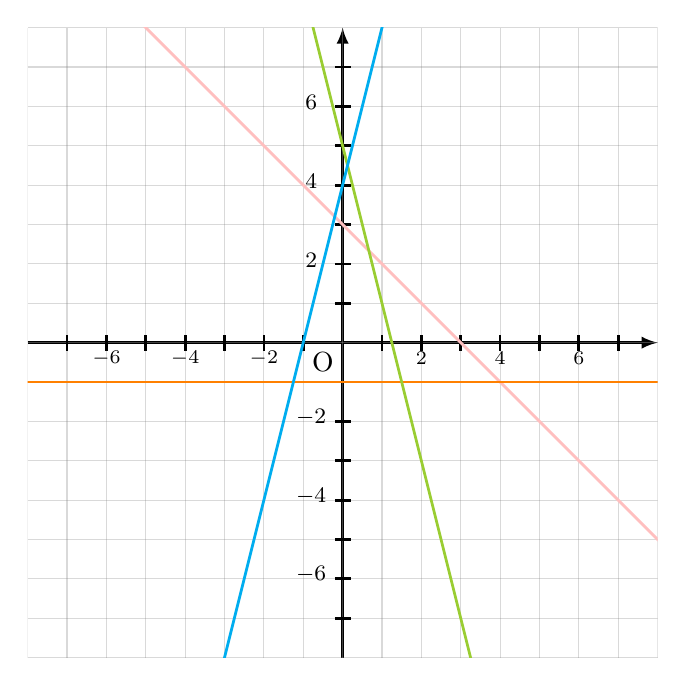
\begin{tikzpicture}[baseline,scale = 0.5]

    \tikzset{
      point/.style={
        thick,
        draw,
        cross out,
        inner sep=0pt,
        minimum width=5pt,
        minimum height=5pt,
      },
    }
    \clip (-8,-8) rectangle (8,8);
    	
	\draw[color ={black},line width = 1,>=latex,->] (-8,0)--(8,0);
	\draw[color ={black},line width = 1,>=latex,->] (0,-8)--(0,8);
	\draw[color ={gray},opacity = 0.3] (-8,0)--(8,0);
	\draw[color ={gray},opacity = 0.3] (-8,1)--(8,1);
	\draw[color ={gray},opacity = 0.3] (-8,2)--(8,2);
	\draw[color ={gray},opacity = 0.3] (-8,3)--(8,3);
	\draw[color ={gray},opacity = 0.3] (-8,4)--(8,4);
	\draw[color ={gray},opacity = 0.3] (-8,5)--(8,5);
	\draw[color ={gray},opacity = 0.3] (-8,6)--(8,6);
	\draw[color ={gray},opacity = 0.3] (-8,7)--(8,7);
	\draw[color ={gray},opacity = 0.3] (-8,8)--(8,8);
	\draw[color ={gray},opacity = 0.3] (-8,0)--(8,0);
	\draw[color ={gray},opacity = 0.3] (-8,-1)--(8,-1);
	\draw[color ={gray},opacity = 0.3] (-8,-2)--(8,-2);
	\draw[color ={gray},opacity = 0.3] (-8,-3)--(8,-3);
	\draw[color ={gray},opacity = 0.3] (-8,-4)--(8,-4);
	\draw[color ={gray},opacity = 0.3] (-8,-5)--(8,-5);
	\draw[color ={gray},opacity = 0.3] (-8,-6)--(8,-6);
	\draw[color ={gray},opacity = 0.3] (-8,-7)--(8,-7);
	\draw[color ={gray},opacity = 0.3] (-8,-8)--(8,-8);
	\draw[color ={gray},opacity = 0.3] (0,-8)--(0,8);
	\draw[color ={gray},opacity = 0.3] (1,-8)--(1,8);
	\draw[color ={gray},opacity = 0.3] (2,-8)--(2,8);
	\draw[color ={gray},opacity = 0.3] (3,-8)--(3,8);
	\draw[color ={gray},opacity = 0.3] (4,-8)--(4,8);
	\draw[color ={gray},opacity = 0.3] (5,-8)--(5,8);
	\draw[color ={gray},opacity = 0.3] (6,-8)--(6,8);
	\draw[color ={gray},opacity = 0.3] (7,-8)--(7,8);
	\draw[color ={gray},opacity = 0.3] (8,-8)--(8,8);
	\draw[color ={gray},opacity = 0.3] (0,-8)--(0,8);
	\draw[color ={gray},opacity = 0.3] (-1,-8)--(-1,8);
	\draw[color ={gray},opacity = 0.3] (-2,-8)--(-2,8);
	\draw[color ={gray},opacity = 0.3] (-3,-8)--(-3,8);
	\draw[color ={gray},opacity = 0.3] (-4,-8)--(-4,8);
	\draw[color ={gray},opacity = 0.3] (-5,-8)--(-5,8);
	\draw[color ={gray},opacity = 0.3] (-6,-8)--(-6,8);
	\draw[color ={gray},opacity = 0.3] (-7,-8)--(-7,8);
	\draw[color ={gray},opacity = 0.3] (-8,-8)--(-8,8);
	\draw[color ={black},line width = 1] (1,-0.2)--(1,0.2);
	\draw[color ={black},line width = 1] (2,-0.2)--(2,0.2);
	\draw[color ={black},line width = 1] (3,-0.2)--(3,0.2);
	\draw[color ={black},line width = 1] (4,-0.2)--(4,0.2);
	\draw[color ={black},line width = 1] (5,-0.2)--(5,0.2);
	\draw[color ={black},line width = 1] (6,-0.2)--(6,0.2);
	\draw[color ={black},line width = 1] (7,-0.2)--(7,0.2);
	\draw[color ={black},line width = 1] (-1,-0.2)--(-1,0.2);
	\draw[color ={black},line width = 1] (-2,-0.2)--(-2,0.2);
	\draw[color ={black},line width = 1] (-3,-0.2)--(-3,0.2);
	\draw[color ={black},line width = 1] (-4,-0.2)--(-4,0.2);
	\draw[color ={black},line width = 1] (-5,-0.2)--(-5,0.2);
	\draw[color ={black},line width = 1] (-6,-0.2)--(-6,0.2);
	\draw[color ={black},line width = 1] (-7,-0.2)--(-7,0.2);
	\draw[color ={black},line width = 1] (-0.2,1)--(0.2,1);
	\draw[color ={black},line width = 1] (-0.2,2)--(0.2,2);
	\draw[color ={black},line width = 1] (-0.2,3)--(0.2,3);
	\draw[color ={black},line width = 1] (-0.2,4)--(0.2,4);
	\draw[color ={black},line width = 1] (-0.2,5)--(0.2,5);
	\draw[color ={black},line width = 1] (-0.2,6)--(0.2,6);
	\draw[color ={black},line width = 1] (-0.2,7)--(0.2,7);
	\draw[color ={black},line width = 1] (-0.2,-1)--(0.2,-1);
	\draw[color ={black},line width = 1] (-0.2,-2)--(0.2,-2);
	\draw[color ={black},line width = 1] (-0.2,-3)--(0.2,-3);
	\draw[color ={black},line width = 1] (-0.2,-4)--(0.2,-4);
	\draw[color ={black},line width = 1] (-0.2,-5)--(0.2,-5);
	\draw[color ={black},line width = 1] (-0.2,-6)--(0.2,-6);
	\draw[color ={black},line width = 1] (-0.2,-7)--(0.2,-7);
	\draw (2,-0.4) node[anchor = center] {\scriptsize \color{black}{$2$}};
	\draw (4,-0.4) node[anchor = center] {\scriptsize \color{black}{$4$}};
	\draw (6,-0.4) node[anchor = center] {\scriptsize \color{black}{$6$}};
	\draw (-2,-0.4) node[anchor = center] {\scriptsize \color{black}{$-2$}};
	\draw (-4,-0.4) node[anchor = center] {\scriptsize \color{black}{$-4$}};
	\draw (-6,-0.4) node[anchor = center] {\scriptsize \color{black}{$-6$}};
	\draw (-0.8,2.1) node[anchor = center] {\footnotesize \color{black}{$2$}};
	\draw (-0.8,4.1) node[anchor = center] {\footnotesize \color{black}{$4$}};
	\draw (-0.8,6.1) node[anchor = center] {\footnotesize \color{black}{$6$}};
	\draw (-0.8,-1.9) node[anchor = center] {\footnotesize \color{black}{$-2$}};
	\draw (-0.8,-3.9) node[anchor = center] {\footnotesize \color{black}{$-4$}};
	\draw (-0.8,-5.9) node[anchor = center] {\footnotesize \color{black}{$-6$}};
	\draw[color={pink},line width = 1] (-35.355328118658136,38.355328118658136)--(36.355328118658136,-33.355328118658136);
	\draw[color={orange},line width = 1] (-50,-1)--(51,-1);
	\draw[color={YellowGreen},line width = 1] (-12.126780150692221,53.507120602768886)--(13.126780150692221,-47.507120602768886);
	\draw[color={cyan},line width = 1] (-12.126780150692221,-44.507120602768886)--(13.126780150692221,56.507120602768886);
	\draw [color={black}] (-0.5,-0.5) node[anchor = center,scale=1, rotate = 0] {O};

\end{tikzpicture}\\\end{minipage}
	

\end{Exercice}

% @see : https://coopmaths.fr/alea?uuid=41e6f&id=2G30-7&n=4&d=10&s=2&alea=ftKt&cd=1&cols=1
\begin{Exercice}
\begin{minipage}[t]{\linewidth} Donner par lecture graphique une équation réduite de chacune des droites ci-dessous.

\medskip
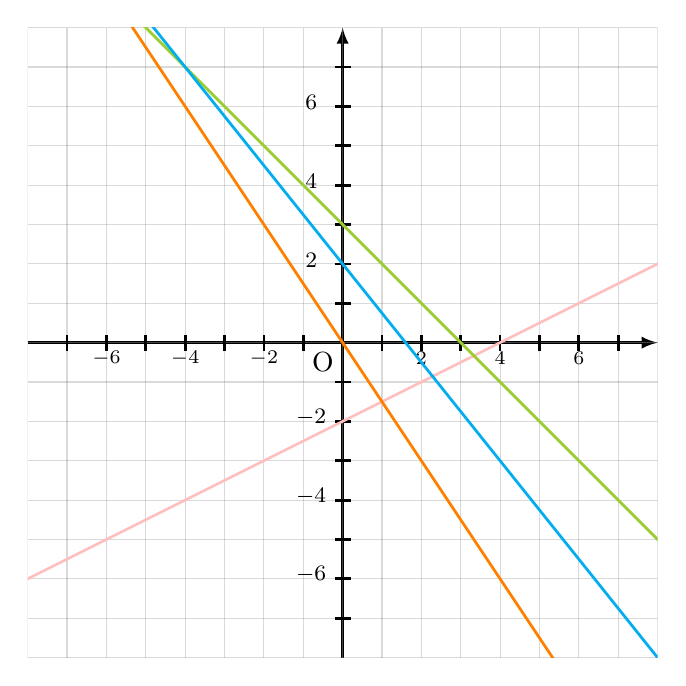
\begin{tikzpicture}[baseline,scale = 0.5]

    \tikzset{
      point/.style={
        thick,
        draw,
        cross out,
        inner sep=0pt,
        minimum width=5pt,
        minimum height=5pt,
      },
    }
    \clip (-8,-8) rectangle (8,8);
    	
	\draw[color ={black},line width = 1,>=latex,->] (-8,0)--(8,0);
	\draw[color ={black},line width = 1,>=latex,->] (0,-8)--(0,8);
	\draw[color ={gray},opacity = 0.3] (-8,0)--(8,0);
	\draw[color ={gray},opacity = 0.3] (-8,1)--(8,1);
	\draw[color ={gray},opacity = 0.3] (-8,2)--(8,2);
	\draw[color ={gray},opacity = 0.3] (-8,3)--(8,3);
	\draw[color ={gray},opacity = 0.3] (-8,4)--(8,4);
	\draw[color ={gray},opacity = 0.3] (-8,5)--(8,5);
	\draw[color ={gray},opacity = 0.3] (-8,6)--(8,6);
	\draw[color ={gray},opacity = 0.3] (-8,7)--(8,7);
	\draw[color ={gray},opacity = 0.3] (-8,8)--(8,8);
	\draw[color ={gray},opacity = 0.3] (-8,0)--(8,0);
	\draw[color ={gray},opacity = 0.3] (-8,-1)--(8,-1);
	\draw[color ={gray},opacity = 0.3] (-8,-2)--(8,-2);
	\draw[color ={gray},opacity = 0.3] (-8,-3)--(8,-3);
	\draw[color ={gray},opacity = 0.3] (-8,-4)--(8,-4);
	\draw[color ={gray},opacity = 0.3] (-8,-5)--(8,-5);
	\draw[color ={gray},opacity = 0.3] (-8,-6)--(8,-6);
	\draw[color ={gray},opacity = 0.3] (-8,-7)--(8,-7);
	\draw[color ={gray},opacity = 0.3] (-8,-8)--(8,-8);
	\draw[color ={gray},opacity = 0.3] (0,-8)--(0,8);
	\draw[color ={gray},opacity = 0.3] (1,-8)--(1,8);
	\draw[color ={gray},opacity = 0.3] (2,-8)--(2,8);
	\draw[color ={gray},opacity = 0.3] (3,-8)--(3,8);
	\draw[color ={gray},opacity = 0.3] (4,-8)--(4,8);
	\draw[color ={gray},opacity = 0.3] (5,-8)--(5,8);
	\draw[color ={gray},opacity = 0.3] (6,-8)--(6,8);
	\draw[color ={gray},opacity = 0.3] (7,-8)--(7,8);
	\draw[color ={gray},opacity = 0.3] (8,-8)--(8,8);
	\draw[color ={gray},opacity = 0.3] (0,-8)--(0,8);
	\draw[color ={gray},opacity = 0.3] (-1,-8)--(-1,8);
	\draw[color ={gray},opacity = 0.3] (-2,-8)--(-2,8);
	\draw[color ={gray},opacity = 0.3] (-3,-8)--(-3,8);
	\draw[color ={gray},opacity = 0.3] (-4,-8)--(-4,8);
	\draw[color ={gray},opacity = 0.3] (-5,-8)--(-5,8);
	\draw[color ={gray},opacity = 0.3] (-6,-8)--(-6,8);
	\draw[color ={gray},opacity = 0.3] (-7,-8)--(-7,8);
	\draw[color ={gray},opacity = 0.3] (-8,-8)--(-8,8);
	\draw[color ={black},line width = 1] (1,-0.2)--(1,0.2);
	\draw[color ={black},line width = 1] (2,-0.2)--(2,0.2);
	\draw[color ={black},line width = 1] (3,-0.2)--(3,0.2);
	\draw[color ={black},line width = 1] (4,-0.2)--(4,0.2);
	\draw[color ={black},line width = 1] (5,-0.2)--(5,0.2);
	\draw[color ={black},line width = 1] (6,-0.2)--(6,0.2);
	\draw[color ={black},line width = 1] (7,-0.2)--(7,0.2);
	\draw[color ={black},line width = 1] (-1,-0.2)--(-1,0.2);
	\draw[color ={black},line width = 1] (-2,-0.2)--(-2,0.2);
	\draw[color ={black},line width = 1] (-3,-0.2)--(-3,0.2);
	\draw[color ={black},line width = 1] (-4,-0.2)--(-4,0.2);
	\draw[color ={black},line width = 1] (-5,-0.2)--(-5,0.2);
	\draw[color ={black},line width = 1] (-6,-0.2)--(-6,0.2);
	\draw[color ={black},line width = 1] (-7,-0.2)--(-7,0.2);
	\draw[color ={black},line width = 1] (-0.2,1)--(0.2,1);
	\draw[color ={black},line width = 1] (-0.2,2)--(0.2,2);
	\draw[color ={black},line width = 1] (-0.2,3)--(0.2,3);
	\draw[color ={black},line width = 1] (-0.2,4)--(0.2,4);
	\draw[color ={black},line width = 1] (-0.2,5)--(0.2,5);
	\draw[color ={black},line width = 1] (-0.2,6)--(0.2,6);
	\draw[color ={black},line width = 1] (-0.2,7)--(0.2,7);
	\draw[color ={black},line width = 1] (-0.2,-1)--(0.2,-1);
	\draw[color ={black},line width = 1] (-0.2,-2)--(0.2,-2);
	\draw[color ={black},line width = 1] (-0.2,-3)--(0.2,-3);
	\draw[color ={black},line width = 1] (-0.2,-4)--(0.2,-4);
	\draw[color ={black},line width = 1] (-0.2,-5)--(0.2,-5);
	\draw[color ={black},line width = 1] (-0.2,-6)--(0.2,-6);
	\draw[color ={black},line width = 1] (-0.2,-7)--(0.2,-7);
	\draw (2,-0.4) node[anchor = center] {\scriptsize \color{black}{$2$}};
	\draw (4,-0.4) node[anchor = center] {\scriptsize \color{black}{$4$}};
	\draw (6,-0.4) node[anchor = center] {\scriptsize \color{black}{$6$}};
	\draw (-2,-0.4) node[anchor = center] {\scriptsize \color{black}{$-2$}};
	\draw (-4,-0.4) node[anchor = center] {\scriptsize \color{black}{$-4$}};
	\draw (-6,-0.4) node[anchor = center] {\scriptsize \color{black}{$-6$}};
	\draw (-0.8,2.1) node[anchor = center] {\footnotesize \color{black}{$2$}};
	\draw (-0.8,4.1) node[anchor = center] {\footnotesize \color{black}{$4$}};
	\draw (-0.8,6.1) node[anchor = center] {\footnotesize \color{black}{$6$}};
	\draw (-0.8,-1.9) node[anchor = center] {\footnotesize \color{black}{$-2$}};
	\draw (-0.8,-3.9) node[anchor = center] {\footnotesize \color{black}{$-4$}};
	\draw (-0.8,-5.9) node[anchor = center] {\footnotesize \color{black}{$-6$}};
	\draw[color={pink},line width = 1] (-44.721359099991595,-24.360679549995798)--(45.721359099991595,20.860679549995798);
	\draw[color={orange},line width = 1] (-27.735004237908647,41.602506356862975)--(28.735004237908647,-43.102506356862975);
	\draw[color={YellowGreen},line width = 1] (-35.355328118658136,38.355328118658136)--(36.355328118658136,-33.355328118658136);
	\draw[color={cyan},line width = 1] (-31.234753535930274,41.043441919912844)--(32.234753535930274,-38.293441919912844);
	\draw [color={black}] (-0.5,-0.5) node[anchor = center,scale=1, rotate = 0] {O};

\end{tikzpicture}\\\end{minipage}

\end{Exercice}

\end{multicols}

\newpage

\subsection*{Systèmes d'équations}

% @see : https://coopmaths.fr/alea?uuid=ccb71&id=2G34-3&n=4&d=10&s=3&alea=VNsp&cd=1&cols=1
\begin{Exercice}
Déterminer si le couple proposé est solution du système d'équations.

\begin{enumerate}[itemsep=1em]
	\item \begin{minipage}[t]{\linewidth} Le couple $(5;-1)$ est-il solution du système $\begin{cases}\begin{aligned}3x+6y &=9\\-x+2y &=13\end{aligned}\end{cases}$ ?\end{minipage}
	\item \begin{minipage}[t]{\linewidth} Le couple $(5;-4)$ est-il solution du système $\begin{cases}\begin{aligned}5x-12y-39 &=x-8y-3\\20x-5y+23 &=17x-y+53\end{aligned}\end{cases}$ ?\end{minipage}
	\item \begin{minipage}[t]{\linewidth} Le couple $(-7;-3)$ est-il solution du système $\begin{cases}\begin{aligned}9x-y-23 &=4x-55\\-x+11y+29 &=4x+6y+49\end{aligned}\end{cases}$ ?\end{minipage}
	\item \begin{minipage}[t]{\linewidth} Le couple $(-6;2)$ est-il solution du système $\begin{cases}\begin{aligned}-9x+14y-8 &=-6x+15y+4\\-5x-10y-31 &=-10x-13y-47\end{aligned}\end{cases}$ ?\end{minipage}
\end{enumerate}
\end{Exercice}

% @see : https://coopmaths.fr/alea?uuid=521b6&id=2G34-7&n=6&d=10&s=3&alea=FBge&cd=1&cols=1
\begin{Exercice}
Résoudre les systèmes suivants par substitution :
\begin{multicols}{3}
\begin{enumerate}[itemsep=1em]
	\item \begin{minipage}[t]{\linewidth}$\begin{cases}\begin{aligned}-3x &=12y-24\\x &=y+3\end{aligned}\end{cases}$\end{minipage}
	\item \begin{minipage}[t]{\linewidth}$\begin{cases}\begin{aligned}2x &=2y-10\\2x &=-y-16\end{aligned}\end{cases}$\end{minipage}
	\item \begin{minipage}[t]{\linewidth}$\begin{cases}\begin{aligned}x &=-y-10\\12x &=3y\end{aligned}\end{cases}$\end{minipage}
	\item \begin{minipage}[t]{\linewidth}$\begin{cases}\begin{aligned}-4y &=12x-24\\y &=-5x+6\end{aligned}\end{cases}$\end{minipage}
	\item \begin{minipage}[t]{\linewidth}$\begin{cases}\begin{aligned}3x &=-3y+42\\x &=4y-16\end{aligned}\end{cases}$\end{minipage}
	\item \begin{minipage}[t]{\linewidth}$\begin{cases}\begin{aligned}-8y &=4x+44\\y &=-x-2\end{aligned}\end{cases}$\end{minipage}
\end{enumerate}
\end{multicols}
\end{Exercice}

% @see : https://coopmaths.fr/alea?uuid=5179b&id=2G34-5&n=6&d=10&s=1&s2=false&s3=false&alea=pYnD&cd=1&cols=1
\begin{Exercice}
Résoudre les systèmes d'équations suivants par combinaison linéaire :
\begin{multicols}{3}
\begin{enumerate}[itemsep=1em]
	\item \begin{minipage}[t]{\linewidth} $\begin{cases}\begin{aligned}-3x+y &=11\\-3x-5y &=53\end{aligned}\end{cases}$\end{minipage}
	\item \begin{minipage}[t]{\linewidth} $\begin{cases}\begin{aligned}-5x-5y &=-20\\5x+y &=16\end{aligned}\end{cases}$\end{minipage}
	\item \begin{minipage}[t]{\linewidth} $\begin{cases}\begin{aligned}4x+5y &=-33\\3x+3y &=-18\end{aligned}\end{cases}$\end{minipage}
	\item \begin{minipage}[t]{\linewidth} $\begin{cases}\begin{aligned}-2x-2y &=-4\\5x-5y &=20\end{aligned}\end{cases}$\end{minipage}
	\item \begin{minipage}[t]{\linewidth} $\begin{cases}\begin{aligned}2x-y &=-1\\2x+6y &=62\end{aligned}\end{cases}$\end{minipage}
	\item \begin{minipage}[t]{\linewidth} $\begin{cases}\begin{aligned}-x+2y &=-21\\-4x-y &=-30\end{aligned}\end{cases}$\end{minipage}
\end{enumerate}
\end{multicols}
\end{Exercice}

\newpage

% @see : https://coopmaths.fr/alea?uuid=fade2&id=2G34-8&n=6&d=10&s=3&alea=bh37&cd=1&cols=1
\begin{Exercice}
Les systèmes suivants ont-ils une, aucune ou une infinité de solutions ?
\vspace{-0.5cm}
\begin{multicols}{3}
\begin{enumerate}[itemsep=1em]
	\item \begin{minipage}[t]{\linewidth} $\begin{cases}\begin{aligned}-6x-6y &=24\\-3x-3y &=12\end{aligned}\end{cases}$\end{minipage}
	\item \begin{minipage}[t]{\linewidth} $\begin{cases}\begin{aligned}-4x+y &=40\\-6x-y &=50\end{aligned}\end{cases}$\end{minipage}
	\item \begin{minipage}[t]{\linewidth} $\begin{cases}\begin{aligned}8x+12y+4 &=2x+6y+4\\5x-4y+14 &=7x-y+20\end{aligned}\end{cases}$\end{minipage}
	\item \begin{minipage}[t]{\linewidth} $\begin{cases}\begin{aligned}3x+4y &=-41\\-3x-4y &=43\end{aligned}\end{cases}$\end{minipage}
	\item \begin{minipage}[t]{\linewidth} $\begin{cases}\begin{aligned}-5x+6y+14 &=-3x+4y-4\\-7x-6y-2 &=-8x-5y+7\end{aligned}\end{cases}$\end{minipage}
	\item \begin{minipage}[t]{\linewidth} $\begin{cases}\begin{aligned}11x+2y-11 &=5x+4y+1\\9x-7 &=6x+y-5\end{aligned}\end{cases}$\end{minipage}
\end{enumerate}
\end{multicols}
\end{Exercice}

% @see : https://coopmaths.fr/alea?uuid=6fbf9&id=2G34-9&n=4&d=10&s=3&alea=jJVE&cd=1&cols=1
\begin{Exercice}
Résourdre les problèmes suivants :

\begin{enumerate}[itemsep=1em]
\item Le périmètre d'un terrain rectangulaire vaut $140\,\text{m}$. Si on augmente la largeur d'un terrain rectangulaire de $20\,\text{m}$ et on 
         augmente la longueur de $18\,\text{m}$, l'aire du terrain augmente de $1710\,\text{m}^2$. \\ Déterminer les mesures du terrain ?
	\item On doit répartir des élèves dans des groupes pour une excursion. Si on met $133$ élèves par groupe, alors on au besoin de $8$ groupes de moins que si on met $77$ élèves par groupe. \\ Combien d'élèves y a-t-il ?
	\item Le périmètre d'un terrain rectangulaire vaut $128\,\text{m}$. Si on diminue la largeur d'un terrain rectangulaire de $6\,\text{m}$ et on 
         diminue la longueur de $13\,\text{m}$, l'aire du terrain diminue de $460\,\text{m}^2$. \\ Déterminer les mesures du terrain ?
	\item On doit répartir des élèves dans des groupes pour une excursion. Si on met $47$ élèves par groupe, alors on au besoin de $18$ groupes de plus que si on met $141$ élèves par groupe. \\ Combien d'élèves y a-t-il ?

\end{enumerate}
\end{Exercice}

% @see : https://coopmaths.fr/alea?uuid=1b828&id=2G34-4&n=3&d=10&s=1&alea=90YD&cd=1&cols=1
\begin{Exercice}
Déterminer le point d' intersection des droites suivantes :

\begin{enumerate}[itemsep=1em]
	\item \begin{minipage}[t]{\linewidth}La droite $d_1$ d'équation $y=3x+6$ et la droite $d_2$ d'équation $y=6x+9$. \end{minipage}
	\item \begin{minipage}[t]{\linewidth}La droite $d_3$ d'équation $y=6x-46$ et la droite $d_4$ d'équation $y=4x-28$. \end{minipage}
	\item \begin{minipage}[t]{\linewidth}La droite $d_5$ d'équation $y=-3x+7$ et la droite $d_6$ d'équation $y=-4x+9$. \end{minipage}
\end{enumerate}
\end{Exercice}

% @see : https://coopmaths.fr/alea?uuid=4b211&id=2G34-12&n=1&d=10&alea=txx1&cd=1&cols=1
\begin{Exercice}

Soient les points $A(-10;-11),\,B(5;-5), \;C(6;3)$ et $D(-6;5)$. \\
Déterminer, s'il existe, le point d'intersection entre la droite $(AB)$ et la droite $(CD)$.
\end{Exercice}

\newpage
% @see : https://coopmaths.fr/alea/?uuid=2eee3&id=2G34-2&n=3&d=10&s=1&cd=1&cols=1&alea=7PPR
\begin{Exercice}
Déterminer la position relative des droites et en déduire le nombre de solutions des systèmes d'équations :
\vspace{-0.5cm}
\begin{multicols}{3}
\begin{enumerate}[itemsep=1em]
	\item \begin{minipage}[t]{\linewidth}$\begin{cases}\begin{aligned}y &=4x-16\\-y &=-4x+16\end{aligned}\end{cases}$\end{minipage}
	\item \begin{minipage}[t]{\linewidth}$\begin{cases}\begin{aligned}-2x &=-y-19\\-2x &=-y-9\end{aligned}\end{cases}$\end{minipage}
	\item \begin{minipage}[t]{\linewidth}$\begin{cases}\begin{aligned}y &=6x-24\\-4y &=-8x+16\end{aligned}\end{cases}$\end{minipage}
\end{enumerate}
\end{multicols}
\end{Exercice}

%https://www.melomaths.fr/static/main/pdfs/2ndNC02systemes_equations-fiche_exercices-corrige.pdf
\begin{Exercice}
Trois amis pêcheurs achètent des poches d'hameçons et des bouchons. Les poches sont toutes au même prix, les bouchons aussi.
\begin{itemize}[label=\textcolor{Couleur6}{$\bullet$}]
\item Le premier prend 3 poches et 2 bouchons.
\item Le second prend 2 poches et 4 bouchons.
\item Le troisième prend 4 poches et 1 bouchon.
\end{itemize} 
Le premier a dépensé 4,60€, le second 6€. \\
Combien a dépensé le troisième?

\end{Exercice}

\begin{Exercice}
Dans un élevage de poules et de lapins, il y a 2 171 têtes et 4 368 pattes.\\
Combien y a-t-il de poules et de lapins?
\end{Exercice}



\begin{Exercice}
Un musée propose un tarif pour les adultes à 7€ et un autre pour les enfant à 4,50€. Lors de cette journée, ce musée a reçu la visites de 205 personnes et la recette totale a été de 1 222,50€.\\
Déterminer le nombre d'adultes puis d'enfants qui ont visité le musée ce jour là. 
\end{Exercice}


\begin{Exercice}
Un marchand de glace vend des glaces à la vanille à 0,50€ l'unité et des glaces au chocolat 0,75€.
\begin{itemize}[label=\textcolor{Couleur6}{$\bullet$}]
\item  À la fin de la journée, il affirme : « Si j'avais vendu les glaces à la vanille 0,75€ et les glaces au chocolat 0,50€, j'aurais fait la même recette : 108,25€ ».
Qu'en pensez-vous?
\item  Le lendemain, n'ayant pas changé ses prix, il affirme : « La recette du jour est de 71,25€. Si j'avais vendu les glaces à la vanille 0,75€ et celles au chocolat 0,50€, j'aurais fait la même recete qu'hier »
\end{itemize}
Qu'en pensez-vous?
\end{Exercice}

\begin{Exercice}
Dans un centre commercial, il y a un tapis de 300 mètres.
Un client marchant à vitesse constante fait l'aller-retour. À l'aller il met 1 minute et 30 secondes. Au retour, à contre-sens, il met 4 minutes et 30 secondes.\\
Déterminer la vitesse du piéton et la vitesse du tapis roulant.
\end{Exercice}
}
